\chapter{Introducción}
\label{ch:intro}

\section{Descripción del problema}
\label{sec:DescripcionProblema}
El objetivo de este trabajo es desarrollar y construir una planta
educativa de control de nivel
(\textit{Level control trainer}).
La planta será utilizada para realizar prácticas con los
alumnos, permitiendo aplicar los conceptos de
control de procesos, programación de \gls{plc}, \gls{scada},
ajuste de lazos PID, teoría de cascadas, etc.
Además, el alumno se familiarizará con elementos de control que
se encuentran en la industria, tales como sensores diferenciales de presión
(\textit{DP cell}), placas orificio y válvulas electroneumáticas.
El proyecto está destinado a ser utilizado por las cátedras de
Automatismos Industriales y Autómatas y Control Discreto de
Ingeniería en Mecatrónica,
como así también Instrumentación y Control Automático de Ingeniería Industrial
y de Petróleos.

En la actualidad, en el Laboratorio de Control Automático de la Facultad, 
se disponen con equipos similares al descripto.
No obstante, el proyecto planteado tiene la característica de ser 
\textbf{móvil}: se encuentra montado en una estructura que 
permite su libre desplazamiento, y el enlace a la
computadora de control se realizará de manera inalámbrica.
Además, se utilizará una válvula electroneumática que cuenta con un
electroposicionador, la primera de su tipo en el laboratorio.

Pueden adquirirse en el mercado plantas educativas de control de nivel, llave
en mano.
Dos firmas del medio fueron consultadas, para conocer 
el precio de un desarrollo similar:
\begin{itemize}
 \item \textbf{Reino Unido}: Una planta con características similares
 a la descripta tiene un precio de $16225\,USD$ en puerto de Buenos Aires.
 \item \textbf{Italia}: Con un precio de $28403\,EUR$ en puerto. 
 El modelo propuesto por la firma italiana
 posee un precio superior debido a que está construido en acero inoxidable.
\end{itemize}

Se observa que el costo llave en mano de un producto de estas características
es muy elevado.
Además, se advierte que muchos de los elementos constitutivos de estas plantas
(sensores, actuadores y autómatas) pueden adquirirse en el mercado, con fines
industriales.
Se plantea entonces el objetivo del proyecto:

\textbf{``Diseñar, ensamblar y programar una planta móvil de control de nivel,
utilizando sensores, controladores y actuadores industriales disponibles en el
mercado''.}

\subsection{Especificaciones}
\label{subsec:especificaciones}

Las siguientes especificaciones deben respetarse para la nueva planta:

\begin{itemize}
\item Debe cumplir su objetivo pedagógico, permitiendo
 a los alumnos comprender los principios del control automático.
 Por consiguiente, la planta no debe ser excesivamente compleja.
 \item Su costo debe ser inferior a una solución llave en mano.
 \item Deberán utilizarse actuadores, elementos de adquisición
 y controladores que se encuentren en plantas industriales.
 \item Tendrá que estar montada sobre una estructura que facilite su
movilidad. Además, deberán evitarse conexiones cableadas, siendo reemplazadas
por enlaces inalámbricos de ser posible.
 \item En ella deberán poder representarse fenómenos que
afectan los procesos industriales, tales como perturbaciones y
tiempos muertos en los procesos.
 \item Deberá verificarse su correcto funcionamiento escribiendo un programa de
ejemplo en el \gls{plc}, con su \gls{scada} correspondiente.
El programa deberá estar correctamente documentado, para que pueda ser
utilizado como ejemplo durante las prácticas.
 \item Un manual de uso sencillo tendrá que ser confeccionado.
 El manual detallará como poner en funcionamiento la planta, especificando las
soluciones a los problemas más comunes que enfrentará el usuario.
\end{itemize}

\section{Materiales disponibles}
\label{sec:MaterialesDisponibles}

A la hora de comenzar con el proyecto, varios elementos habían
sido adquiridos por el director de proyecto y se encontraban
disponibles en el Laboratorio de Control Automático:
\begin{itemize}
  \item \textbf{Estructura:} un marco de caño estructural montado sobre
  ruedas. En él se colocarán todos los elementos de la planta.
  Ver Sec. \ref{sec:EstructuraSoporte}.

  \item \textbf{Cañerías y accesorios}: serán utilizados para realizar el
  circuito hidráulico de la planta. Ver Sec. \ref{sec:Canerias}.

  \item \textbf{Tanques:} se trata de dos caños cloacales sellados en sus
  extremos, de $200\,mm$ de diámetro. Ver Sec. \ref{sec:Tanques}.

  \item \textbf{Electrobombas monofásicas (2):} impulsarán el fluido
  en el circuito hidráulico.
  La velocidad de las bombas (frecuencia) no será controlada.
  Ver Sec. \ref{sec:Bombas}.

  \item \textbf{Válvula electroneumática:} marca Foxboro, modelo
  Stabilflo (serie V1), para controlar el caudal.
  Se trata de una válvula isoporcentual, con un electroposicionador
  Power Genex.
  La apertura de la válvula será nuestra variable manipulada en
  el sistema.
  Ver Sec. \ref{sec:ValvulaNeumatica}.

  \item \textbf{Placa orificio:} permite medir el
  caudal en una tubería midiendo la diferencia de presión generada por una 
  reducción del diámetro de la cañería. Ver Sec. \ref{subsec:PlacaOrificio}.

  \item \textbf{DP cells (2):} sensores de presión
  diferencial Yokogawa, modelo \verb|EJA 110 A|.
  Uno de los sensores será utilizado para medir el nivel del tanque controlado,
  en tanto que el segundo medirá caudal con la ayuda de la placa orificio.
  Ver Sec. \ref{subsec:DPCell}.

  \item \textbf{Manómetros (2):} A colocar en
  puntos específicos de la planta, para medir los valores instantáneos de
  presión.
  Ver Sec. \ref{subsec:Manometros}.

  \item \textbf{Instrumentos de protección y comando:}
  se dispone de un interruptor magnetotérmico de corte general,
  Sec. \ref{subsec:corteGeneral}.
  Para las bombas, podemos citar: contactores, relés y los relevos térmicos.
  Ver Sec. \ref{subsec:alimentacionMotores}.

  \item \textbf{Fuente de alimentación:}
  de $220\,V$ en corriente alterna a $24\,V$ en corriente continua.
  Permite alimentar el \gls{plc} y el módulo inalámbrico (previa conversión a
  $5\,V$ en corriente continua).
  Ver Sec. \ref{subsec:fuenteAlim}.

  \item{\textbf{\gls{plc}}}: Twido \verb|40 DTK| (Schneider) con un módulo
  analógico \verb|TWD AMM 6HT|.
  Permitirá controlar las bombas (encendido/apagado), 
  leer valores de presión de las DP Cell y modificar la apertura de la 
  válvula. Ver Sec. \ref{subsec:plc}.

  \item \textbf{Módulos inalámbricos:} marca CTM Electrónica,
  modelo \verb|AD-200|.
  Permite enlazar la interfaz \verb|RS 485| a la computadora de control
  de manera inalámbrica. Ver Sec. \ref{subsec:inalambrico}.
\end{itemize}

A partir de los materias disponibles, se confeccionó
un proyecto de trabajo, estableciendo las tareas a realizar, la jerarquía de
tareas y un planning de trabajo.

\section{Solución propuesta}
\label{sec:SolucionPropuesta}

Habiendo analizado la lista de materiales disponibles, se propone el siguiente
modelo de planta de control de nivel:
\begin{itemize}
 \item Dos tanques son alimentados por dos bombas centrífugas.
 Cada bomba extraerá agua de un tanque y lo enviará al otro.
 \item En uno de ellos, el \textbf{tanque controlado}, se medirá el nivel
 mediante un DP cell.
 \item Sobre la \textbf{cañería de llenado} del tanque controlado, se
 colocará la válvula electroneumática y la placa orificio (junto
con su correspondiente DP cell)\footnote{Si bien no es  requisito contar con
una placa orificio para hacer  control de nivel,  poder medir el caudal en la
cañería de llenado resulta  de  interés para  futuros trabajos  utilizando
Teoría de Cascadas.}.
 Por ende, puede controlarse con precisión el caudal de agua de llenado del
 tanque controlado (de ahí su nombre).
 \item En el segundo tanque, el \textbf{tanque de reserva} no se medirá
 el  nivel, sino que será estimado indirectamente mediante el nivel del tanque
 controlado.
 \item En la \textbf{cañería de vaciado} del tanque controlado se colocará una
válvula manual, que permitirá modificar el caudal de vaciado.
\end{itemize}


Para poder recrear fenómenos que afectan los procesos industriales se agregarán
los siguientes elementos a la planta:
\begin{itemize}
\item 20 metros de cañería adicional, que sirven como tiempo
muerto.
Se agregarán en paralelo de la cañería de llenado del tanque controlado.
Se podrá habilitar el tiempo muerto mediante una válvula manual.

\item Se realizará la conexión, mediante una válvula manual, de la salida de
cada bomba con su entrada. Mediante esta conexión se podrá modificar el
rendimiento de las bombas para lograr el balance de masa en la planta, como así
también simular perturbaciones en el circuito hidráulico.

\end{itemize}

Una explicación completa del diseño e implementación del circuito hidráulico
propuesto se realiza en el Cap. \ref{ch:DisenoEnsamblado}.

Luego de la instalación del circuito hidráulico, deben cablearse los elementos
de protección y comando de los motores.
Además, se propone controlar la planta utilizando un autómata
programable (\gls{plc}).
La válvula electroneumática, el comando de las bombas y los sensores de presión
deben ser correctamente conectados en el tablero de control.
El cableado se analiza en el Cap. \ref{ch:tablero}.

En el Cap. \ref{ch:progPLC} se programará el autómata que controlará la
planta. Finalmente, en el Cap. \ref{ch:scada} se desarrollará el software
de control \gls{scada}, que se ejecuta en la computadora de control.

\section{Análisis económico}
\label{sec:AnalisisEconomico}
Los elementos descriptos en la Sec. \ref{sec:MaterialesDisponibles} fueron
obtenidos mediante donaciones para el proyecto.
Distinguimos tres donantes:
\begin{itemize}
 \item \textbf{Techint:} donó el \gls{plc} (con su módulo analógico y fuente),
las celdas de presión diferencial, las electrobombas y la válvula de control.
Esta donación está especificada en detalle en la Tab.
\ref{tab:donacionTechint}.
 \item \textbf{La Facultad de Ingeniería:} donó la estructura, la cañería, los
accesorios, las válvulas manuales, los manómetros, los elementos de ferretería,
los elementos de electricidad (contactores, relés) y el módulo inalámbrico.
El detalle de la donación puede observarse en la Tab. \ref{tab:donacionFing}.
\item \textbf{El director de proyecto, Ing. Puglesi:} donó la placa orificio,
necesaria para poder medir el caudal en la cañería de llenado.
El detalle de la donación puede observarse en la Tab.
\ref{tab:donacionPuglesi}.
\end{itemize}

Aunque los elementos fueron donados, se realizará el análisis de costos de la
planta para compararlo con las soluciones llave en mano descriptas en
\ref{sec:DescripcionProblema}.
El precio de cada uno de los elementos fue calculado en dólares estadounidenses
(USD) para evitar posibles fluctuaciones de precio en la moneda local (ARS).

El costo total de la planta es de
\begin{align}
5050\,USD + 2122\,USD + 50\,USD &= 7222\,USD
\end{align}
Se verifica que el precio es inferior a las soluciones llave en mano, para un
producto con una calidad similar\footnote{Comparando con la firma inglesa,
que propone una planta de calidad similar. Recordemos que, si bien la planta
italiana es más costosa, estaba construida en acero inoxidable.}.

Cabe destacar que en nuestro análisis no hemos tenido en cuenta el costo (en
horas de trabajo) para realizar el proyecto.
\begin{table}[!t]
\renewcommand{\arraystretch}{1.3}
\centering
\begin{tabularx}{\textwidth}{l||X||l}
\hline
\bfseries Cantidad & \bfseries Descripción &\bfseries Precio\\
\hline \hline
2& Electrobombas monofásicas Czerweny 1/4 HP &
 {\multirow{6}{*}{5050 USD}}\\
1& \gls{plc} Twido \texttt{40 DTK} &  \\
1& Módulo 4E-2S analógicas \texttt{TWD AMM 6HT}& \\
2& Celdas de presión diferencial Yokogawa \texttt{E 110 A}& \\
1& Válvula electroneumática de control & \\
1& Fuente de poder $220\,V$ AC a $24\,V$ CC& \\
\hline
\end{tabularx}
\caption{Elementos donados por Techint}
\label{tab:donacionTechint}
\end{table}

\begin{table}[!t]
\renewcommand{\arraystretch}{1.3}
\centering
\begin{tabularx}{\textwidth}{l||X||l}
\hline
\bfseries Cantidad & \bfseries Descripción & \bfseries Precio\\
\hline \hline
1& Estructura móvil con tablero&
 {\multirow{9}{*}{2122 USD}}\\
-& Tuberías y accesorios &  \\
2& Columnas (tanques) &  \\
-& Elementos de ferretería (bulones, tuercas, etc.)& \\
-& Material eléctrico &\\
2& Manómetros& \\
3& Válvulas exclusas manuales& \\
3& Válvulas globo manuales& \\
1& Módulo inalámbrico \texttt{AD-200}&\\
\hline
\end{tabularx}
\caption{Elementos donados por la Facultad de Ingeniería}
\label{tab:donacionFing}
\end{table}

\begin{table}[!t]
\renewcommand{\arraystretch}{1.3}
\centering
\begin{tabularx}{\textwidth}{l||X||l}
\hline
\bfseries Cantidad & \bfseries Descripción & \bfseries Precio\\
\hline \hline
1& Placa Orificio& 50 USD\\
\hline
\end{tabularx}
\caption{Elementos donados por el Ing. Puglesi}
\label{tab:donacionPuglesi}
\end{table}

\section{Organización}
\label{sec:Organizacion}
\subsection{División del trabajo}
Dado que la construcción de la planta implica una serie de etapas que
deben realizarse de manera ordenada, se dividió el trabajo en los siguientes
puntos:
\begin{enumerate}
 \item \textbf{Planificación y diseño preliminar}
  \item \textbf{Construcción de la planta}
  \begin{enumerate}
   \item Preparación de la estructura
   \item Montaje de los elementos de la planta
   \item Cañerías
   \item Cableado eléctrico de potencia
   \item Cableado de señal: PLC, válvula, DP cells, módulo inalámbrico.
   \item Pruebas de funcionamiento sencillas
   \item Pintura y acabados
  \end{enumerate}
  \item \textbf{Programación del \gls{plc}}
  \item \textbf{Programación del software SCADA}
  \item \textbf{Pruebas de funcionamiento}
  \item \textbf{Documentación}
\end{enumerate}

\subsection{Planning}
Se optó por dividir el tiempo disponible en cada una de las tareas, tal como lo
explicita el planning propuesto en la Fig. \ref{fig:EDT}.
Se observa que la mayor parte de las actividades de construcción de la planta
debieron realizarse de manera seriada, en tanto que la programación del
\gls{plc} y el \gls{scada} puede realizarse de forma paralela.
\begin{figure}[ht!]
	\centering
	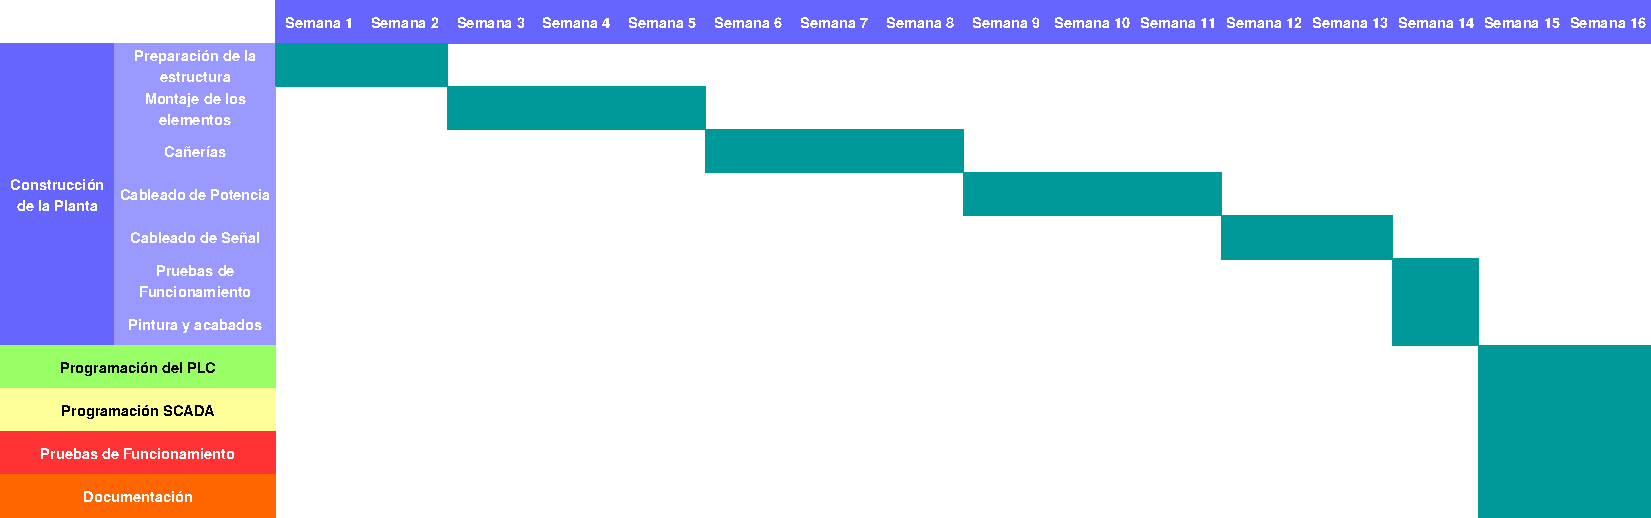
\includegraphics[angle=90,
		width=0.501\textwidth]{Cap1-Introduccion/images/EDT.pdf}
	\caption{Esquema de la división del tiempo por semanas.}
	\label{fig:EDT}
\end{figure}

% REVISIÓN 1 - fclad
